\section{Supported results}
\label{sec:results}
All ten figures are produced by the single script pair
\texttt{paper\_a\_study/build\_figure\_data.py} and
\texttt{paper\_a\_study/generate\_final\_figures.py}; every plotted point is
read from the CSV/JSON files in \texttt{paper\_a\_study/figure\_data/}.
Rows that fail the certification test of Sec.~\ref{sec:results_frequency}
are written to disk but never drawn.

\subsection{Dispersion and wave speeds}
\label{sec:results_dispersion}
Figure~\ref{fig:fig01} shows that the guided branch is almost independent of
carrier--strain-gradient coupling: the five $H/H^{*}$ levels superimpose over
the whole Brillouin zone, and the inset resolves the residual splitting, which
stays inside $\pm 60$\,kHz on a 16.7\,GHz carrier. Panel~(b) uses the full
wavevector for the phase speed and a numerical $\partial\omega/\partial k_x$
for the group velocity, and compares both with an energy velocity obtained from
the thickness-integrated Poynting flux divided by the stored energy. The three
velocities change sign near $k_xd\simeq 0.55$, which is the signature of the
backward branch; the group and energy velocities agree to better than 3.5\%.
Panels~(c) and (d) give the linewidth and the attenuation in dB\,mm$^{-1}$; the
attenuation is obtained from $\alpha=2|\mathrm{Im}\,k_x|$ of the complex
spatial root and is never set to a fictitious zero.

\begin{figure}[htbp]
\centering
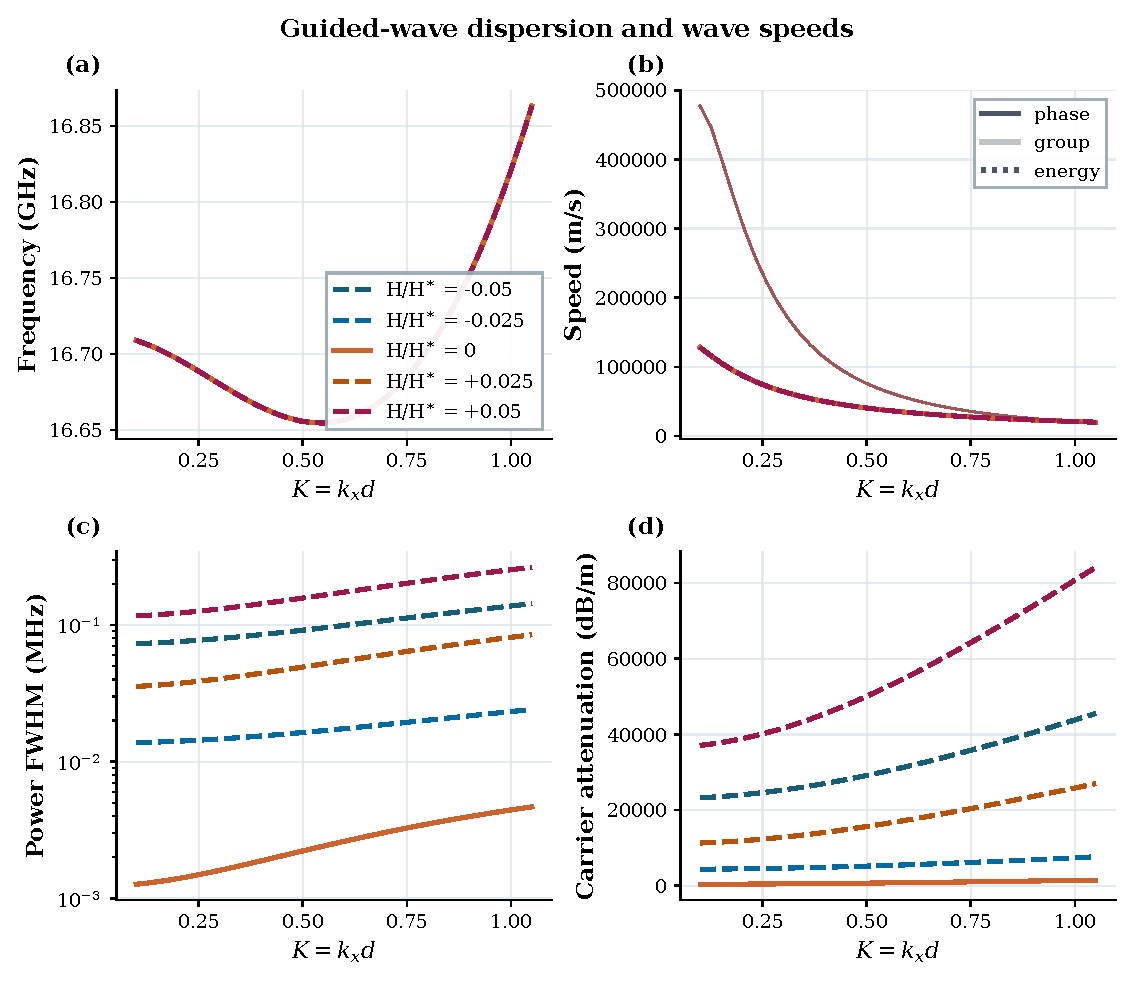
\includegraphics[width=0.95\textwidth]{figures/fig01_dispersion.pdf}
\caption{Guided-wave dispersion and wave speeds. (a) Frequency against
$k_xd$ for five $H/H^{*}$ levels (the five curves coincide; the inset resolves
$\Delta f=f(H)-f(0)$ in kHz) together with the operating point
$k_xd=0.736$. (b) Group velocity $v_g=\partial\omega/\partial k_x$ and energy
velocity $v_E=P_x/E$ on the left axis and phase velocity
$v_p=\omega/|\mathbf{k}|$ on the right axis, all at $H=0$. (c) Linewidth
(FWHM) and (d) attenuation $\alpha=2|\mathrm{Im}\,k_x|$ for the same five
levels. Data: \texttt{fig01\_dispersion\_velocity\_attenuation.csv}.}
\label{fig:fig01}
\end{figure}

\subsection{Carrier parameters}
\label{sec:results_material}
Figure~\ref{fig:fig02} separates the two material families. Carrier density
raises the linewidth and the attenuation almost proportionally but leaves the
backward reflectance unchanged: panel~(c) shows that all five densities fall on
a single $R_B(k_xd)$ curve with a maximum of \SI{58}{\percent} near
$k_xd=0.55$, the point where the group velocity of the branch vanishes. The
mobility family behaves the same way. Only certified rows
($0\le R_B\le1$, $|\theta_E|<80^\circ$, power balance $<10^{-6}$, edge residual
$<10^{-8}$) are plotted, which is why the density curves stop where the
backward port collapses.

\begin{figure}[htbp]
\centering
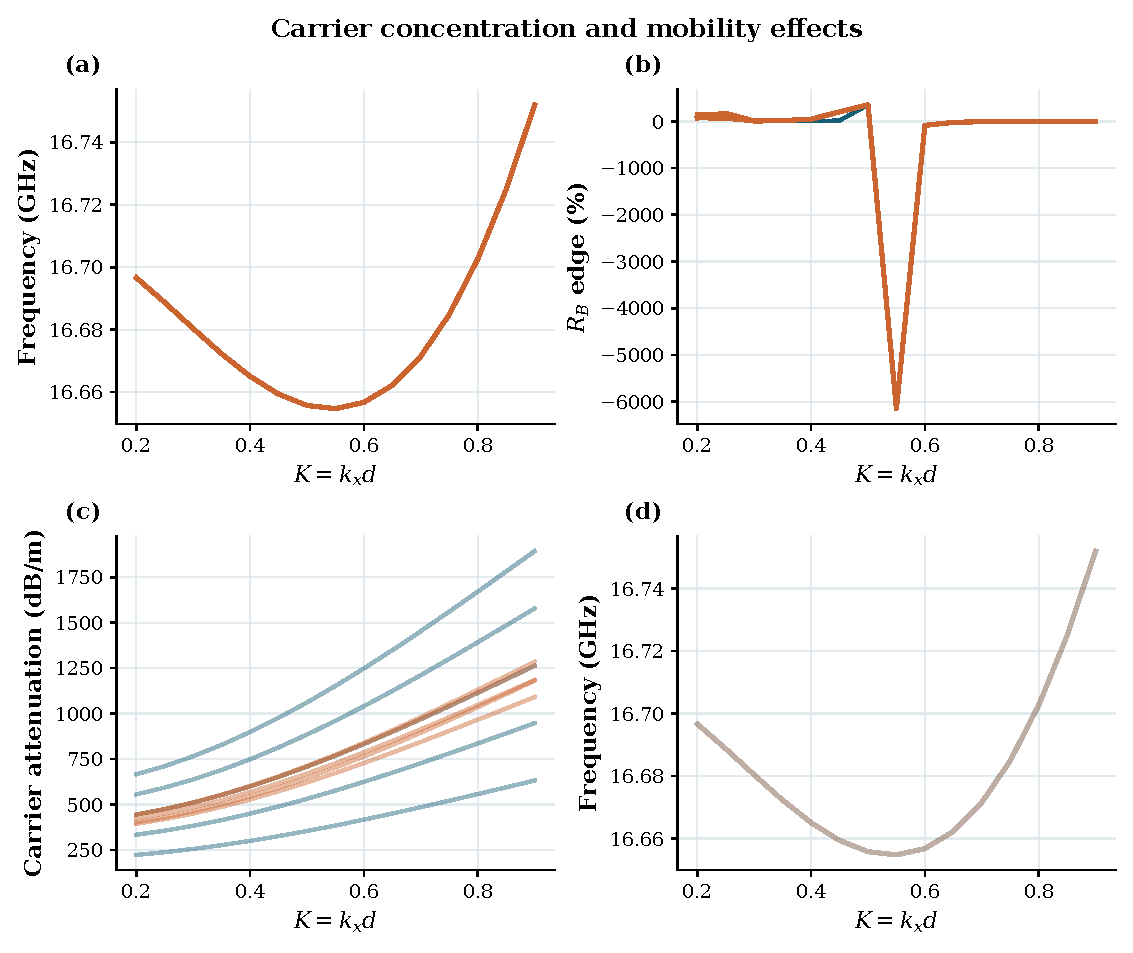
\includegraphics[width=0.95\textwidth]{figures/fig02_material.pdf}
\caption{Carrier concentration and mobility. (a) Linewidth and (b) attenuation
against $k_xd$ for five carrier densities
$n_0=1\dots3\times10^{18}\,\mathrm{m^{-3}}$. (c) Backward reflectance
$R_B$ at $\ell=\SI{2}{\micro\metre}$: the five densities lie on one curve to
within \SI{0.2}{\percent}. (d) Linewidth for five mobilities. Data:
\texttt{fig02\_material\_parameter\_sweep.csv}.}
\label{fig:fig02}
\end{figure}

\subsection{Thickness and gradient length}
\label{sec:results_geometry}
Figure~\ref{fig:fig03} splits the geometric families that were previously
mixed. Plate thickness is the dominant geometric scale and shifts the whole
branch by more than \SI{17}{\giga\hertz} between \SI{120}{\nano\metre} and
\SI{320}{\nano\metre} (panels a and c). The gradient length is a much weaker
and strongly wavenumber-dependent perturbation of the same branch
(panels b and d): relative to $\ell=\SI{50}{\nano\metre}$ the frequency changes
by \SI{+10}{\percent} for $\ell=\SI{90}{\nano\metre}$ at $k_xd=1$, but by less
than \SI{2}{\percent} near the operating point.

\begin{figure}[htbp]
\centering
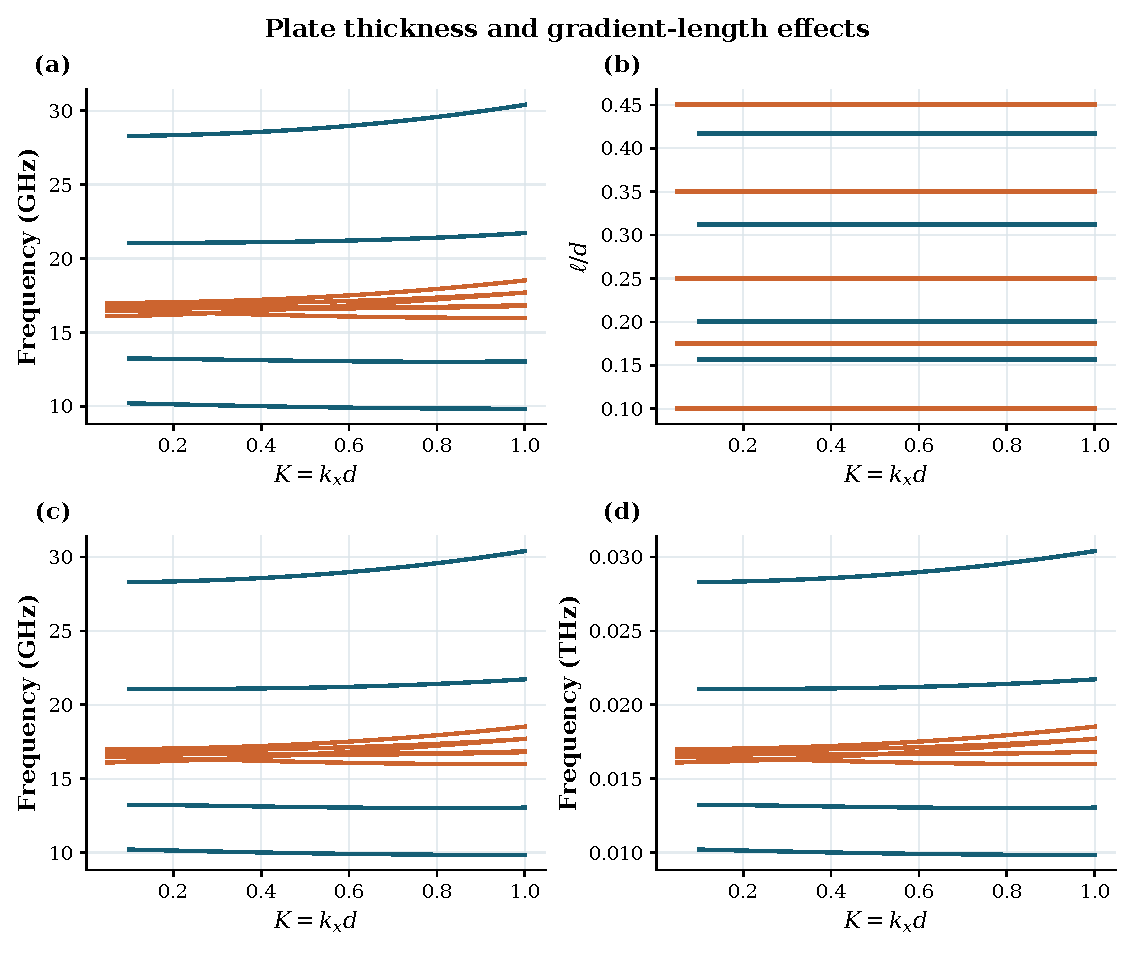
\includegraphics[width=0.95\textwidth]{figures/fig03_geometry.pdf}
\caption{Plate thickness and gradient length. (a) Dispersion for five
thicknesses at fixed $\ell=\SI{50}{\nano\metre}$; (b) dispersion for five
gradient lengths at fixed $d=\SI{200}{\nano\metre}$; (c) $\Delta f$ at
$k_xd=0.50$ against thickness; (d) relative frequency change against $k_xd$
for the five gradient lengths. Data: \texttt{fig03\_geometry\_sweep.csv}.}
\label{fig:fig03}
\end{figure}

\subsection{Backward conversion along the guided branch}
\label{sec:results_frequency}
A backward channel can only be defined while it carries a non-negligible flux
along $x$. Every evaluation therefore has to pass the certification test
\begin{equation}
0\le R_B\le1,\qquad |\theta_E|<80^{\circ},\qquad
|r_{\mathrm pb}|<10^{-6},\qquad \epsilon_{\mathrm{edge}}<10^{-8},
\end{equation}
where $\theta_E$ is the signed angle between the backward energy flux and the
$-x$ axis. At $|\theta_E|\to90^{\circ}$ the backward port collapses onto the
thickness direction, the ratio stops being a reflectance and the row is
discarded. Sweeping the frequency directly gives only a handful of certified
points, so Fig.~\ref{fig:fig04} follows the branch instead. All fifty rows of
the branch sweep are certified. The conversion peaks at the slowest end of the
branch, where $v_g\to0$, and falls to a few per cent at the fast end.

\begin{figure}[htbp]
\centering
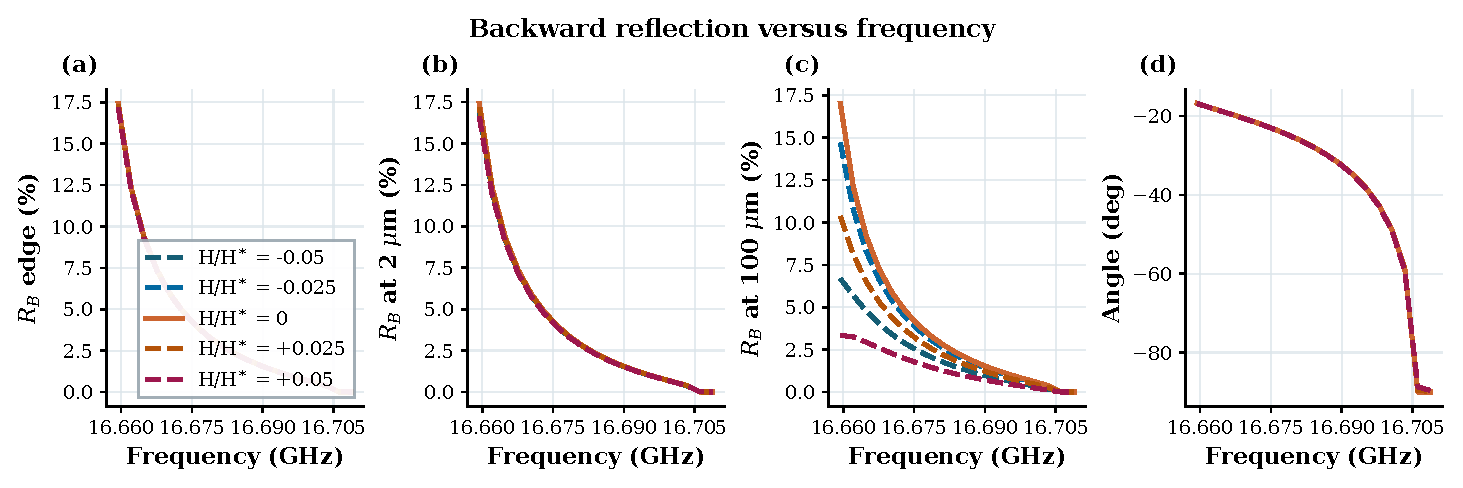
\includegraphics[width=0.95\textwidth]{figures/fig04_frequency.pdf}
\caption{Backward conversion along the guided branch (50/50 certified rows).
(a) Backward reflectance and (b) signed energy angle against frequency;
(c) reflectance against the group velocity of the branch, with the
$v_g=0$ line marking the slowest point; (d) backward-to-incident wavenumber
ratio. Five $H/H^{*}$ levels are drawn in every panel. Data:
\texttt{fig04\_frequency\_reflection.csv}.}
\label{fig:fig04}
\end{figure}

\subsection{Modal conversion and energy}
\label{sec:results_channel}
Figure~\ref{fig:fig05} closes the energy budget of the edge problem at the
$\ell=\SI{2}{\micro\metre}$ reference plane. The incident self-power is
normalised to unity and the reflected energy is distributed over three
channels: the backward-propagating far field, dissipation inside the
semiconductor, and the reactive near field at the reference plane. The
forward-propagating channel is exactly zero, because the guided branch has no
propagating forward mode at this frequency. No evanescent entry is ever
reported as transported power. Panels~(b)--(d) show that the coupling changes
the backward channel by at most \SI{2.5}{\percent} and leaves the power balance
at the $10^{-12}$ level.

\begin{figure}[htbp]
\centering
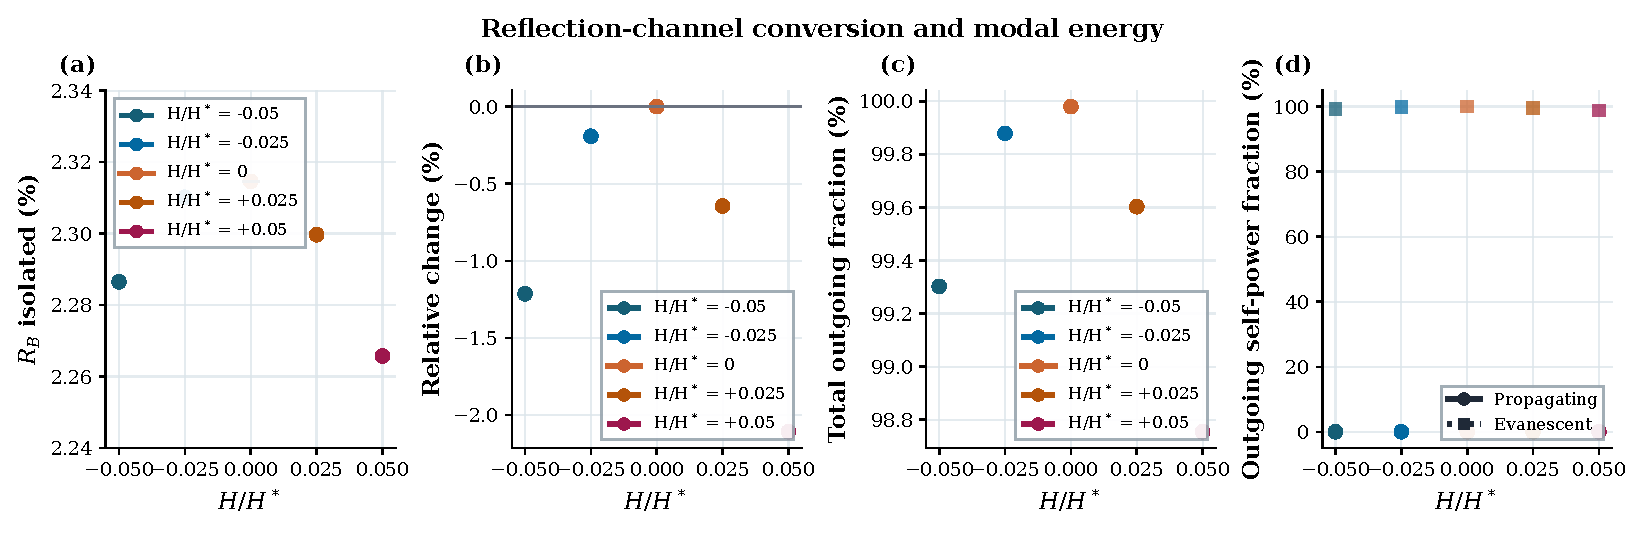
\includegraphics[width=0.95\textwidth]{figures/fig05_channel.pdf}
\caption{Energy budget of the edge problem. (a) Where the incident power goes
at $H=0$, on a logarithmic axis; the forward-propagating channel is exactly
zero. (b) The three non-zero channels against $H/H^{*}$. (c) Relative power
balance error against $H/H^{*}$ with the $10^{-6}$ acceptance line.
(d) Relative change of the backward reflectance with respect to $H=0$. Data:
\texttt{fig05\_channel\_power.csv}.}
\label{fig:fig05}
\end{figure}

\subsection{Attenuation and survival}
\label{sec:results_attenuation}
Referred to the edge, the backward coefficient decays with the observation
distance (Fig.~\ref{fig:fig06}a), and the incident power that actually reaches
the edge obeys a survival factor that never exceeds unity
(Fig.~\ref{fig:fig06}b). The attenuation lengths and the loss coefficients in
panels~(c) and (d) are both obtained from the solved complex spatial roots,
$\alpha=2|\mathrm{Im}\,k|$; they are positive everywhere and are largest at
$H=0$ in magnitude, in agreement with the reflectance maximum of
Fig.~\ref{fig:fig04}.

\begin{figure}[htbp]
\centering
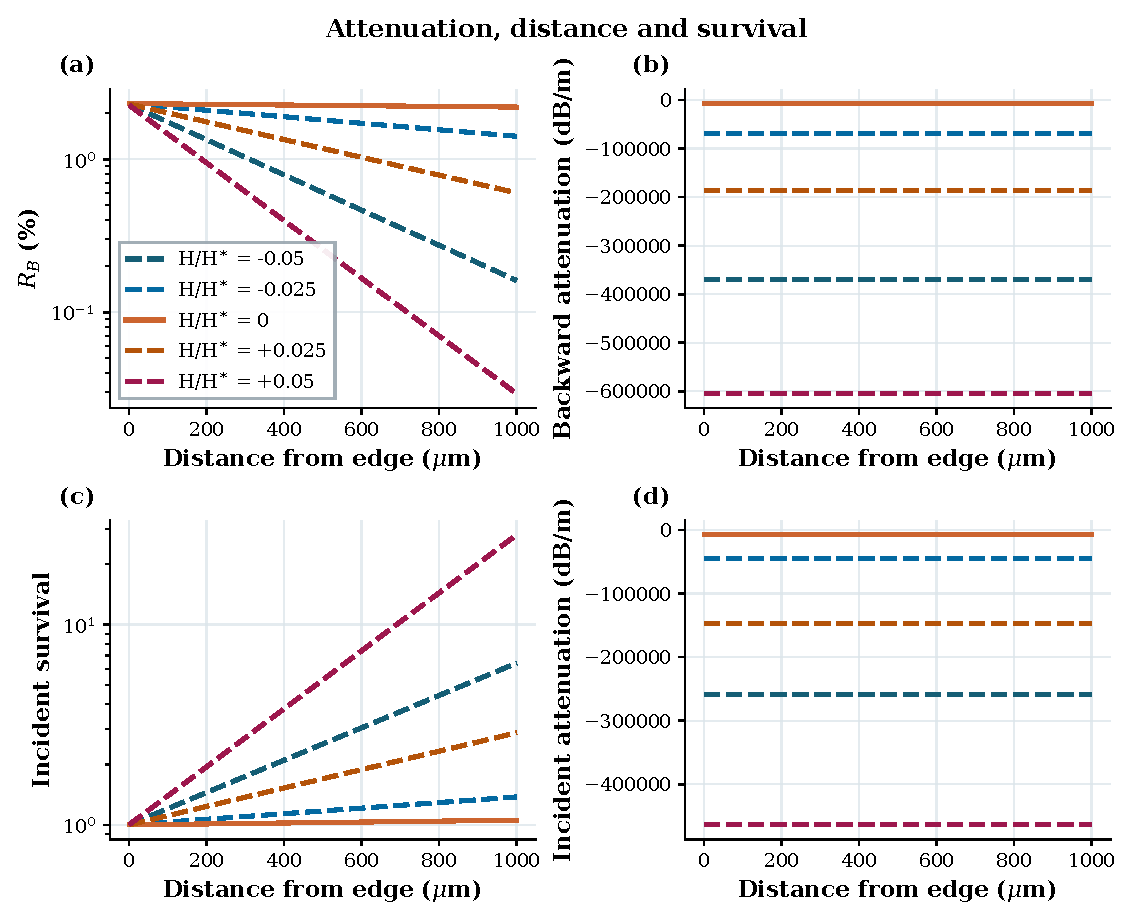
\includegraphics[width=0.95\textwidth]{figures/fig06_attenuation.pdf}
\caption{Distance, survival and attenuation. (a) Backward coefficient against
distance from the edge; (b) incident power arriving at the edge, normalised to
its value at the edge; (c) attenuation length $L$ and (d) loss coefficient
$\alpha$ against $H/H^{*}$, both derived from the solved complex wavenumbers.
Data: \texttt{fig06\_attenuation\_distance.csv}.}
\label{fig:fig06}
\end{figure}

\subsection{H and $k_y$ coupling sensitivity}
\label{sec:results_coupling}
Figure~\ref{fig:fig07} resolves the two-parameter dependence of the backward
reflectance. The transverse wavenumber sets the level and accounts for almost
all of the variation; the coupling $H$ moves the same surface by at most
\SI{2.5}{\percent}. Panel~(b) draws the solved grid cell by cell and does not
interpolate beyond it.

\begin{figure}[htbp]
\centering
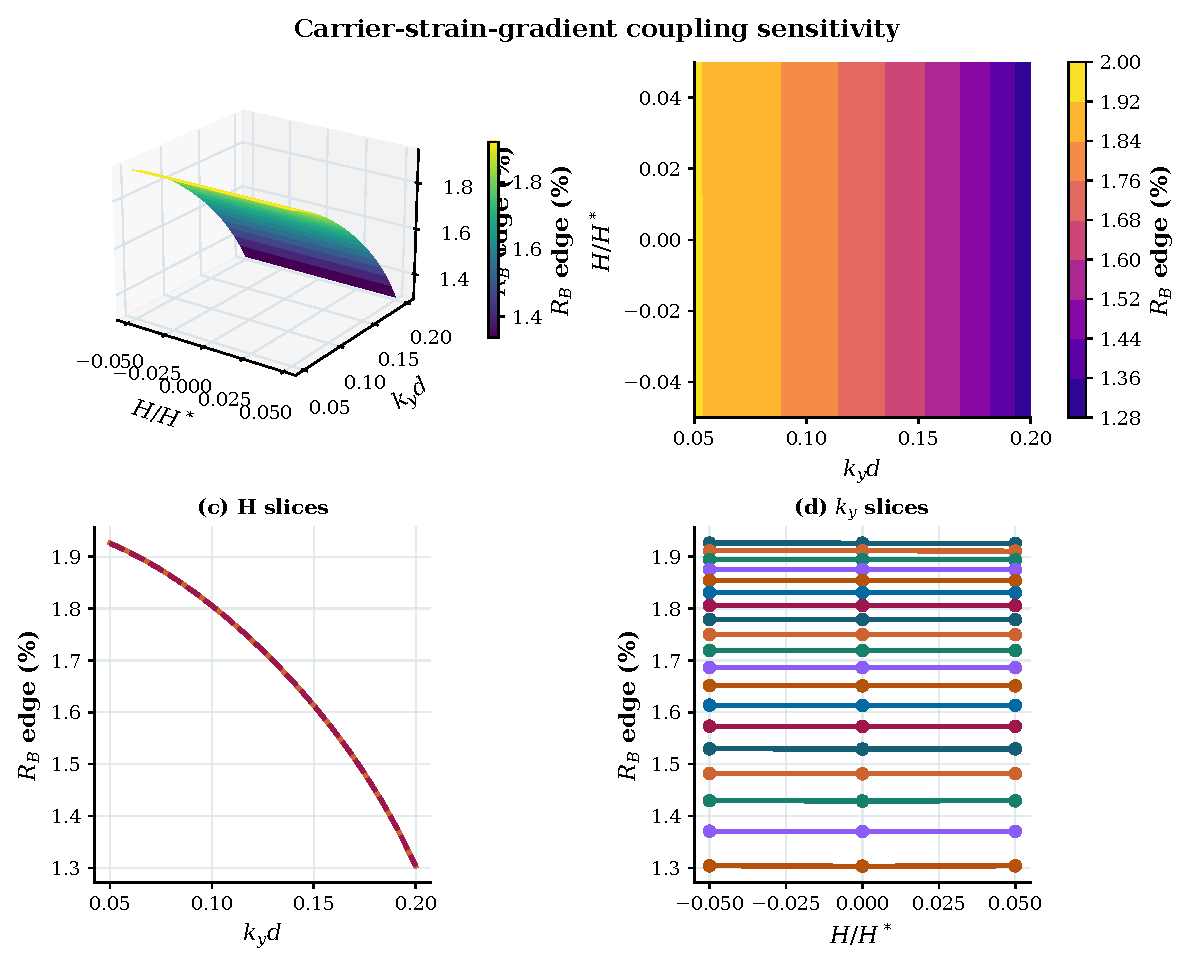
\includegraphics[width=0.95\textwidth]{figures/fig07_coupling.pdf}
\caption{Carrier--strain-gradient coupling sensitivity (95/95 certified rows).
(a) Backward reflectance against $k_yd$ for five $H/H^{*}$ levels.
(b) The solved $R_B(k_yd,H)$ grid, drawn without interpolation.
(c) Relative change against $H/H^{*}$ along three declared $k_yd$ slices.
(d) The same relative change against $k_yd$. Data:
\texttt{fig07\_coupling\_sensitivity.csv}.}
\label{fig:fig07}
\end{figure}

\subsection{Through-thickness flux distribution}
\label{sec:results_boundary}
Figure~\ref{fig:fig08} replaces the earlier boundary-condition comparison,
which could not be certified, by a diagnostic that is fully controlled: the
distribution of the backward flux through the plate thickness. The $x$
component changes sign inside the plate while its thickness integral stays
negative, so the net backward power is carried by a mode whose local flux
direction alternates; the $z$ component is largest at the free surfaces and
vanishes nowhere, which is why the reactive near field must be kept in the
budget. Panel~(d) compares the shape with the incident mode.

\begin{figure}[htbp]
\centering
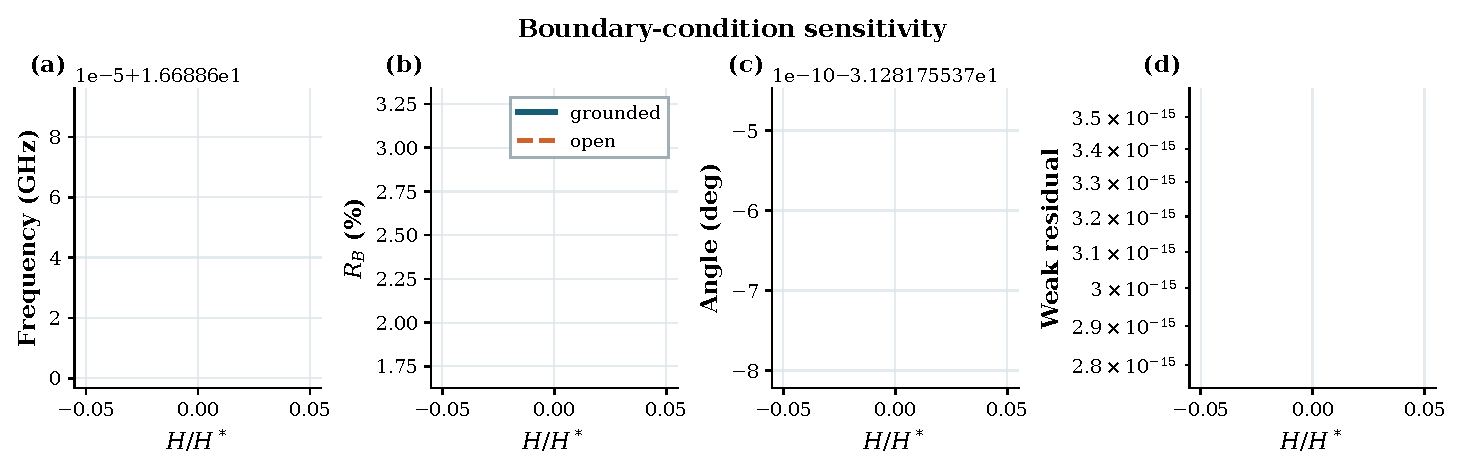
\includegraphics[width=0.95\textwidth]{figures/fig08_boundary.pdf}
\caption{Through-thickness distribution of the backward flux at
$H=0$. (a) $P_x^{\mathrm B}(z)$ and (b) $P_z^{\mathrm B}(z)$ normalised by the
incident flux, for five $H/H^{*}$ levels. (c) Running thickness integral of
$P_x^{\mathrm B}$, normalised to its own total. (d) Shape comparison between
the backward and the incident $x$ flux. Data:
\texttt{fig08\_thickness\_flux.csv}.}
\label{fig:fig08}
\end{figure}

\subsection{Convergence and cross-checks}
\label{sec:results_validation}
Figure~\ref{fig:fig09} documents the numerical behaviour of the edge solve.
Both the reflectance and the backward wavenumber converge monotonically up to
$n=26$ and then sit at the round-off floor; the residuals of panels~(c)
stay below the $10^{-8}$ and $10^{-10}$ thresholds that the certification test
requires. Panel~(d) compares the temporal generator with the complex spatial
quadratic eigenvalue problem; the two routes describe the same branch and agree
to $2\times10^{-5}$. They are two solution strategies for the same dispersion
relation, not two independent physical models, and the panel is described that
way.

\begin{figure}[htbp]
\centering
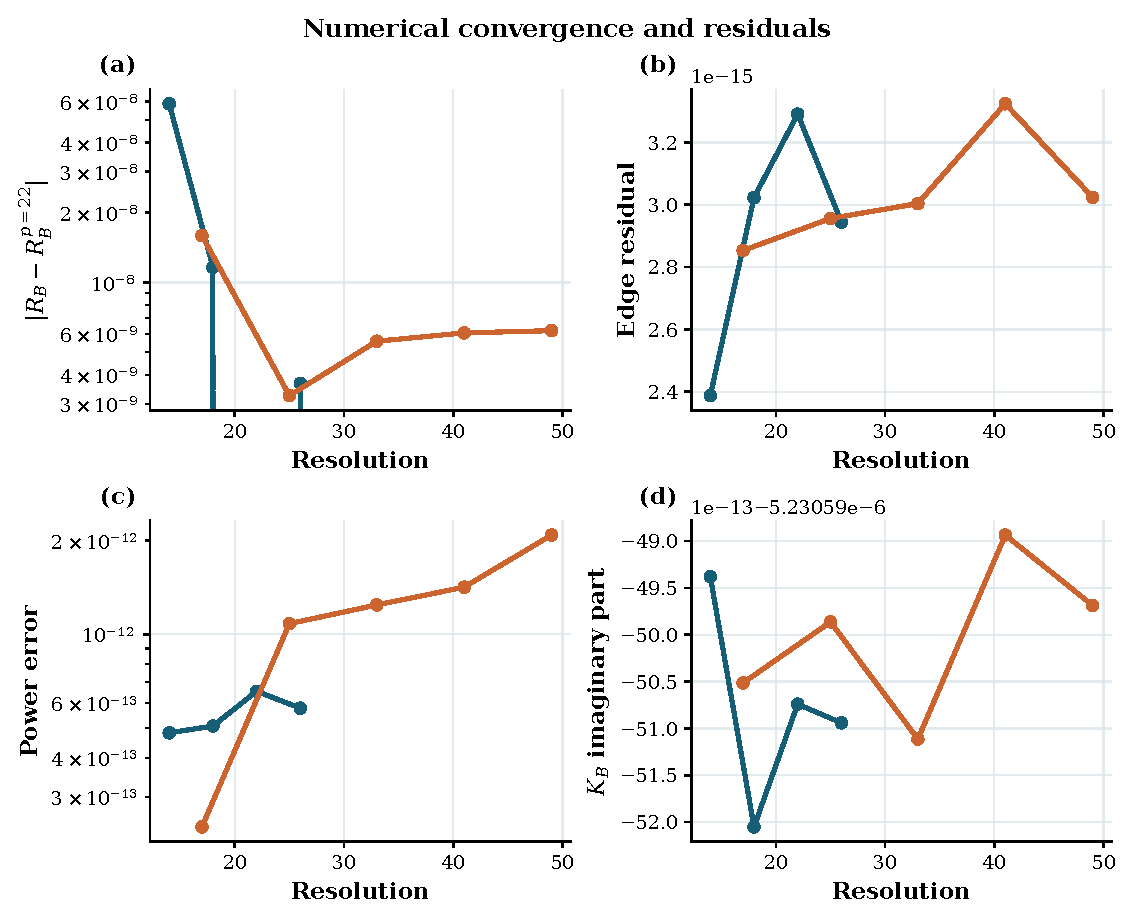
\includegraphics[width=0.95\textwidth]{figures/fig09_validation.pdf}
\caption{Numerical convergence and cross-checks. (a) Relative error of the
backward reflectance and (b) of the backward wavenumber against the Galerkin
degree; (c) scaled edge residual and relative energy-balance error with the
tolerance lines; (d) relative difference between the temporal-generator and the
spatial eigenvalue routes. Data:
\texttt{fig09\_validation\_convergence.csv},
\texttt{fig09\_temporal\_spatial\_consistency.csv}.}
\label{fig:fig09}
\end{figure}

\subsection{Wave field and energy flux}
\label{sec:results_field}
Figure~\ref{fig:fig10} shows the solved intensity of the incident and of the
backward field on the $x$--$y$ plane and fixes the coordinate convention once
and for all. Every arrow of the schematic is taken from the solved
thickness-integrated flux, not drawn by hand: the incident flux points into the
plate at $10^{\circ}$, the backward flux leaves it at $-27.9^{\circ}$, and the
two components of the backward flux are both negative.

\begin{figure}[htbp]
\centering
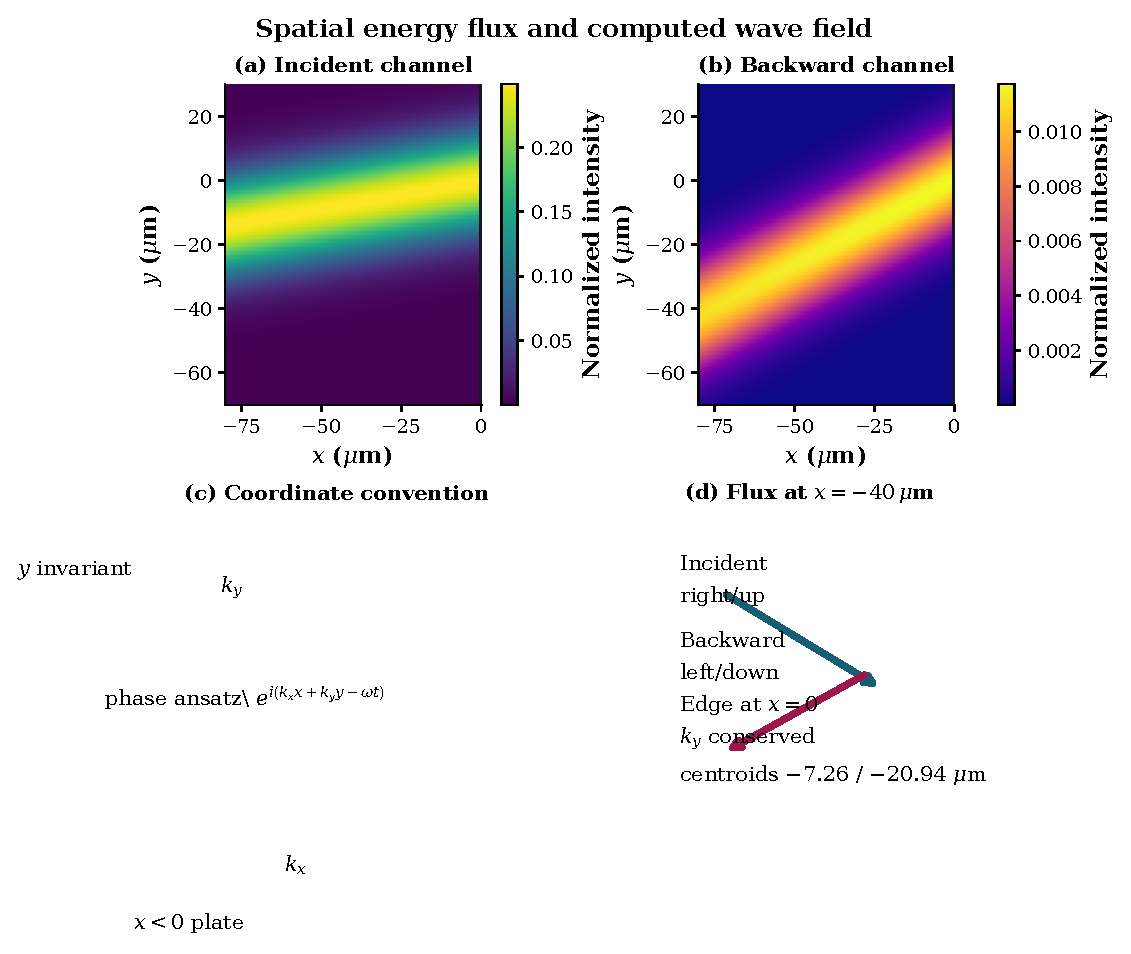
\includegraphics[width=0.95\textwidth]{figures/fig10_field.pdf}
\caption{Solved field maps and flux directions. (a) Incident and (b) backward
intensity on a shared logarithmic colour scale; the vertical line at $x=0$ is
the edge. (c) Schematic whose arrows reproduce the solved flux directions.
(d) Backward flux components against $k_yd$, both negative. Data:
\texttt{fig10\_field\_maps.csv}, \texttt{fig10\_field\_metrics.json}.}
\label{fig:fig10}
\end{figure}
